\documentclass[10pt,landscape]{article}
\usepackage{multicol}
\usepackage{calc}
\usepackage{ifthen}
\usepackage[landscape]{geometry}
\usepackage{hyperref}
\usepackage{graphicx}

% To make this come out properly in landscape mode, do one of the following
% 1.
%  pdflatex Filename.tex
%
% 2.
%  latex Filename.tex
%  dvips -P pdf  -t landscape Filename.dvi
%  ps2pdf Filename.ps


% This sets page margins to .5 inch if using letter paper, and to 1cm
% if using A4 paper. (This probably isn't strictly necessary.)
% If using another size paper, use default 1cm margins.
\ifthenelse{\lengthtest { \paperwidth = 11in}}
	{ \geometry{top=.5in,left=.5in,right=.5in,bottom=.5in} }
	{\ifthenelse{ \lengthtest{ \paperwidth = 297mm}}
		{\geometry{top=1cm,left=1cm,right=1cm,bottom=1cm} }
		{\geometry{top=1cm,left=1cm,right=1cm,bottom=1cm} }
	}

% Turn off header and footer
\pagestyle{empty}
 

% Redefine section commands to use less space
\makeatletter
\renewcommand{\section}{\@startsection{section}{1}{0mm}%
                                {-1ex plus -.5ex minus -.2ex}%
                                {0.5ex plus .2ex}%x
                                {\normalfont\large\bfseries}}
\renewcommand{\subsection}{\@startsection{subsection}{2}{0mm}%
                                {-1explus -.5ex minus -.2ex}%
                                {0.5ex plus .2ex}%
                                {\normalfont\normalsize\bfseries}}
\renewcommand{\subsubsection}{\@startsection{subsubsection}{3}{0mm}%
                                {-1ex plus -.5ex minus -.2ex}%
                                {1ex plus .2ex}%
                                {\normalfont\small\bfseries}}
\makeatother

% Define BibTeX command
\def\BibTeX{{\rm B\kern-.05em{\sc i\kern-.025em b}\kern-.08em
    T\kern-.1667em\lower.7ex\hbox{E}\kern-.125emX}}

% Don't print section numbers
\setcounter{secnumdepth}{0}


\setlength{\parindent}{0pt}
\setlength{\parskip}{0pt plus 0.5ex}


% -----------------------------------------------------------------------

\begin{document}

\raggedright
\footnotesize
\begin{multicols}{3}


% multicol parameters
% These lengths are set only within the two main columns
%\setlength{\columnseprule}{0.25pt}
\setlength{\premulticols}{1pt}
\setlength{\postmulticols}{1pt}
\setlength{\multicolsep}{1pt}
\setlength{\columnsep}{2pt}

\begin{center}
     \Large{\textbf{Algorithm Cheat Sheet}} \\
\end{center}


\newlength{\MyLen}
%\settowidth{\MyLen}{\texttt{letterpaper}/\texttt{a4paper} \ }


\section{Asymptotics}
\begin{tabular}{@{}|    l|@{\ }  l   l  l   l    l| } % 
	$f(n) = ?$ & o & O & $\Theta$ &  $\Omega$ &  $\omega$ \\
	$f(n)/g(n)$ & 0 & $\le$ & $[c_1, c_2]$ & $\ge c$  &  $\infty$ \\
\end{tabular}

\subsection{Loop Invariant}
Initialization
Maintenance
Termination

\section{Solving Recurrences}

\subsection{Master Theorem}
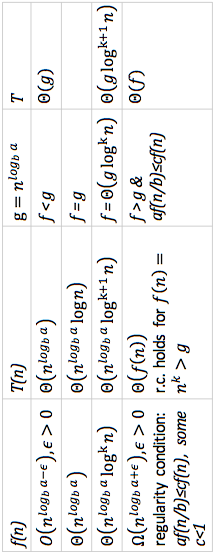
\includegraphics[scale = 0.6]{MT2.png}

\subsection{Simplified}

$T(n) = aT(n/b) + cn$

\begin{tabular}{@{}| l| l| l| @{}} 
	$a<b$ & $a = b$ & $a>b$\\
	$O(n)$ & $O(n\log n) $ & $O(n^{\log_b a})$
\end{tabular}

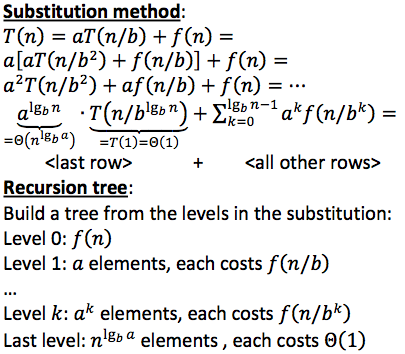
\includegraphics[scale = 0.5]{Recurrences.png}


\section{Quicksort}

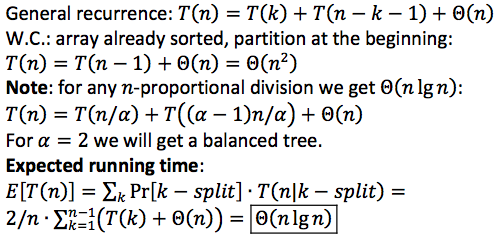
\includegraphics[scale=0.5]{quicksort.png}

\section{Selection}
\textbf{RANDOMIZED-SELECT(A,p,r,i)}
\\q = RANDOMIZED-PARTITION(A,p,r)
\\RANDOMIZED-SELECT(A,q+1,r,i-k)
\\
%Instuctor's manual, P127


\underline{Expected running time}

$X_k = $ I \{subarray $A[p..q]$ has exactly $ k $ eles \}

$T(n) \le \sum_{k=1}^n X_k \cdot (T(\max(n-k, k-1)) +O(n)  ) $

\subsection{Deterministic Selection Algorithm}

%\vspace{-4pt}

\begin{enumerate} \itemsep 0pt
	\item 	Divide A into groups of 5 elements 
	\item 	Find the median in each group (within 7 cmps) $\rightarrow$ subset M
	\item 	Recursively select the median x of M
	\item 	Partition A with respect to pivot x
	\\ 	at least $ 3n/10-6 $ eles are $ \le/\ge x$
	\item 	Recurse on the appropriate part
	\\ $T(n) \le T(\lceil \frac{n}{5} \rceil ) + T(\frac{7n}{10} + 6) + \Theta(n) = O(n)$
\end{enumerate}

\section{Search Tree}


\textbf{TREE-SUCCESSOR(x)}
\\if right[x] $\ne$ NIL
\\\quad then return TREE-MINIMUM(right[x])
\\y $ \gets $ p[x]
\\\textit{//find 1st left parent}
\\while \textbf{y $\ne$ NIL} and x = right[y] do
\\\quad x  $\gets $ y
\\\quad y $ \gets $ p[y]
\\return y

\section{Btree}

	k keys \& k+1 children
	\\\#children [t, 2t]. (root except: [2, 2t]
	\\All leaves at same depth
	\\Leaves: same restriction on \#keys
	\\$ h=\Theta(\log ⁡n/\log ⁡t ) $


If absorb red nodes into their black parents $\rightarrow$ 2-3-4 tree. Red-Black trees can be mapped to a 2-3-4 tree and vice-versa



\section{Red-Black Trees}

%\vspace*{-5pt}
\begin{itemize} \itemsep 0pt
	\item Children, parent of a red node are black
	\item root \& leaves(NIL) is black
	\item All black paths have same \# of blacks (black height)
	\item $  h\le2\log⁡(n+1) $
	The subtree rooted at any node $ x $ contains $ \le 2bh(x) - 1 $ internal nodes. (by induction on $ h $, $ 	bh \le h/2 $
\end{itemize}

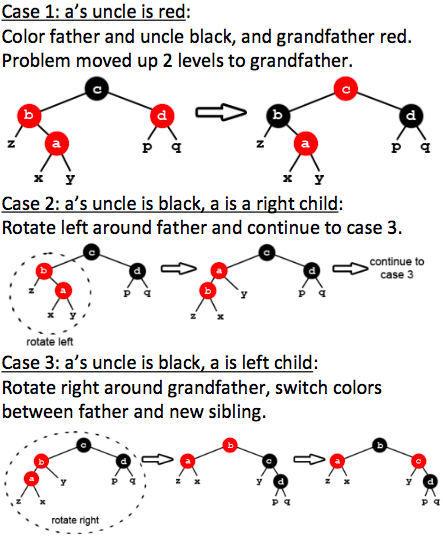
\includegraphics[scale=0.5]{RBtree.png}


\textbf{RB-INSERT(T, z)}
\\\quad y = T.NIL //
\\\quad x = T.root
\\\quad while $x \ne T.NIL$ do
\\\quad \quad y = x
\\\quad \quad if z.key < x.key then
\\\quad \quad \quad x = x.left
\\\quad \quad else x = x.right
\\\quad z.p = y
\\\quad z.left = T.NIL //
\\\quad z.right = T.NIL //
\\\quad z.color = RED //
\\\quad if y == T.NIL then
\\\quad \quad T.root = z
\\\quad elseif z.key < y.key then
\\\quad \quad y.left = z
\\\quad else 
\\\quad \quad y.right = z
\\\quad RB-INSERT-FIXUP(T, z)//

\subsection{delete}

		Determine which y to splice out: either z: no/one child or z's successor.

		x: NIL or a non-NIL child of y

		y is removed by manipulating pointers of p[y] and x. (when y is root!
		
		if y $ \ne $ z, copy its data into z (y is successor)

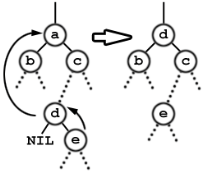
\includegraphics[scale=0.5]{treedel2.png}

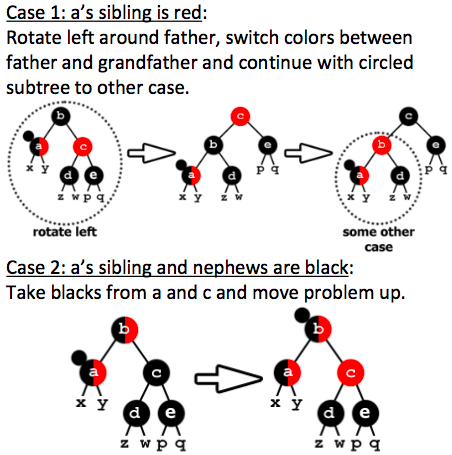
\includegraphics[scale=0.5]{RBdelete1.png}
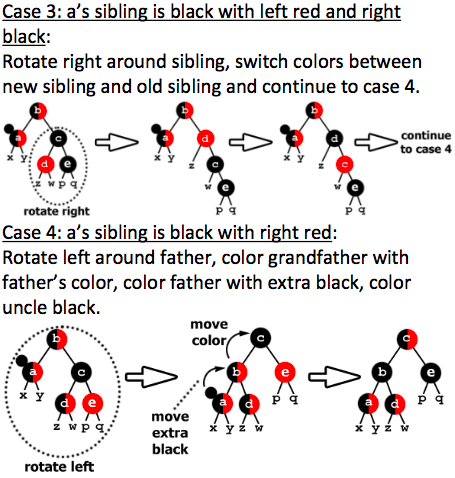
\includegraphics[scale=0.5]{RBdelete2.png}


\section{Examples}

\textbf{PARTITION (A,p,r) }
\\\quad x = A[r]
\\\quad i = p-1
\\\quad for j=p to r-1
\\\quad \quad if $A[j] \le x$ then 
\\\quad \quad \quad i=i+1, swap(A[i],A[j])
\\\quad swap(A[i+1],A[r])
\\\quad return i+1


\textbf{HEAPSORT(A,n)}
\\BUILD-MAX-HEAP(A,n)
\\for $ i \gets n $ downto 2 do
\\\quad exchange $ A[1] \& A[i] $
\\\quad MAX-HEAPIFY(A,1,i −1)

Top $ k $: Compute k largest in sorted order in time $ O(n+k\log n) $
Find $ k $ largest in online stream: $ n\gg k $ elements using space $ O(k) $ in $ O(n\log k) $ time


\textbf{Merge}
\\i=1, j=1
\\for t = 1 to $n_1+n_2$
\\\quad if ($i\le n_1$ and $(j>n_2 \mathrm{\ or\ } K[i]<L[j])$) then
\\\qquad M[t] = K[i], i = i+1
\\\quad else M[t] = L[j], j = j+1 

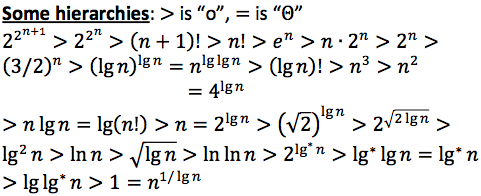
\includegraphics[scale=0.5]{asymptotic.png}
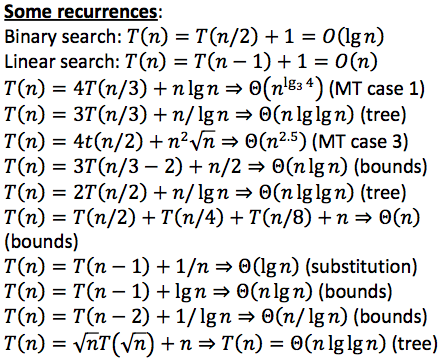
\includegraphics[scale=0.5]{recurrence.png}


\section{Sorting in Linear Time}

\subsection{Comparison lower bounds}
\begin{itemize}
	\item Stirling's formula: $n! = \sqrt{2\pi n} (n/e)^n (1+\Theta(1/n)) $
	\item Simultaneous max and min: ${\lceil 3n/2\rceil}  - 2$
\end{itemize}

% Proving Lower Bounds
% http://web.cs.ucdavis.edu/~amenta/w04/dis2.pdf


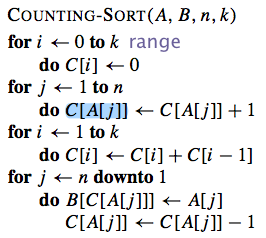
\includegraphics[scale=0.5]{countsort.png}

$\Theta(n+k)$. Auxiliary storage: $ C[0..k] $


\subsection{Radix Sorting}

$\Theta(d(n+k))$.
	
	For n b-bit numbers ($ n\le 2^b $), can partition into blocks of r bits, $ r\le b \Rightarrow \Theta((b/r)(n+2^r )) $
	
	Optimal: $ r\approx \log ⁡n \Rightarrow \Theta(bn/\log⁡ n ) $


\rule{0.3\linewidth}{0.25pt}
\scriptsize

Copyright \copyright\ 2015 Radon Co

%\href{http://www.stdout.org/~winston/latex/}{http://www.stdout.org/$\sim$winston/latex/}


\end{multicols}
\end{document}


% 2008-04
% Changed page margin code to use the geometry package. Also added code for
% conditional page margins, depending on paper size. Thanks to Uwe Ziegenhagen
% for the suggestions.

% 2006-08
% Made changes based on suggestions from Gene Cooperman. <gene at ccs.neu.edu>


% To Do:
% \listoffigures \listoftables
% \setcounter{secnumdepth}{0}


%\subsection{Font size}
%\setlength{\columnsep}{14pt} % Need to move columns apart a little
%\begin{multicols}{2}
%   \begin{tabbing}
%       \verb!\footnotesize!          \= \kill
%       \verb!\tiny!                  \>  \tiny{tiny} \\
%       \verb!\scriptsize!            \>  \scriptsize{scriptsize} \\
%       \verb!\footnotesize!          \>  \footnotesize{footnotesize} \\
%       \verb!\small!                 \>  \small{small} \\
%       \verb!\normalsize!            \>  \normalsize{normalsize} \\
%       \verb!\large!                 \>  \large{large} \\
%       \verb!\Large!                 \=  \Large{Large} \\  % Tab hack for new column
%       \verb!\LARGE!                 \>  \LARGE{LARGE} \\
%       \verb!\huge!                  \>  \huge{huge} \\
%       \verb!\Huge!                  \>  \Huge{Huge}
%   \end{tabbing}
%\end{multicols}
%\setlength{\columnsep}{1pt} % Set column separation back
%
%\verb!{\small! \ldots\verb!}!, or without braces
